\chapter{Un exemple d'application du profil \emph{Game Genesis}~: Le jeu PUBG}

\EH{Tout le chapitre est à revoir avec les nouveaux modèles etc.}

PUBG est un jeu vidéo, sorti en 2017, qui compte d\'ej\`a des millions d'adeptes à travers le globe. Développé par \emph{PUBG Corporation} (filiale de B\emph{luehole, Inc.}, plus récemment de \emph{Krafton Game Union}), PUBG est un des premiers jeux \emph{standalone}%
\footnote{Standalone : Logiciel informatique qui peut s'exécuter de manière indépendante}
%
, avec  \emph{Fortnite} (\emph{Epic Games}),
permettant aux joueurs de participer à un <<\emph{Last man standing game}>>. Ces deux jeux ont été les premiers \emph{standalone} à populariser le \emph{Battle Royale} et à le mettre à la portée de tous sans devoir développer ou installer du contenu additionnel dans des jeux existants.

\gt{Des mods!?}


\section{L'origine des jeux \emph{Battle Royale}}

\gt{Ci-bas: Donner aussi une r\'ef\'erence bibliographiqu pour le roman.}

\gt{Ci-bas: je ne comprends pas <<50 classes de troisi\`eme>>!?}

Les jeux de type \emph{Battle Royale} trouvent leurs racines dans le roman <<\emph{Battle Royale}>>~\cite{takami2003battle} et son adaptation cinématographique.%
%
\footnote{\url{https://www.imdb.com/title/tt0266308}}
%
En gros, l'histoire va comme suit.
Un programme militaire de simulation de combat a lieu dans une République socialiste d'Extrême-Orient complètement coupée du monde extérieur, extrêmement stable politiquement, o\`u les habitants n'ont aucun droit civique. Le programme militaire d\'ebute par un tirage au sort annuel de 50 classes d'élèves de troisième année. La classe tirée au cort est alors déplacée chacune vers une zone de combat. Au début de l'expérience, tous les élèves sont réunis afin de recevoir un briefing rapide, puis se voient attribuer un sac contenant un seul objet (par ex., arme à feu, arme blanche, fourchette, corde de luth, etc). Les \'el\`eves sont ensuite transport\'es et livrés à eux-mêmes dans une zone donnée en ayant pour seule consigne qu'aucune règle n'est imposée\ldots\ et qu'un seul survivant par groupe pourra être gagnant de l'expérience;  les autres devront être exterminés, et ce par n'importe quel moyen. Le champion obtient alors le droit de vivre aux frais de l'État pour le reste de ses jours et la reconnaissance comme <<~Héros du pays~>>.

\section{L'essor de la popularité du \emph{Battle Royale}}
Bien que connu depuis l'ann\'ee 2000, l'intérêt pour le principe du \emph{Battle Royale} n'explose que plus tard, avec le succès de la saga \emph{Hunger Games}%
%
\footnote{\url{https://www.imdb.com/title/tt1392170/}}
%
, mettant en place l'histoire de Katniss Everdeen, une jeune adulte qui participe de son plein gré aux \emph{Hunger Games}. Dans un état totalitaire séparé en castes regroupées dans des districts, deux enfants ou adolescents sont choisis au hasard dans chaque district afin de devenir les Tribus. Ils sont alors réunis dans la capitale et lâchés dans une arène afin de participer à une télé-réalité de match à mort diffusée partout dans le pays.

Le succès des \emph{Hunger Games} a amené les développeurs du jeu \emph{Arma II} à créer un mode de jeu basé sur les mêmes règles. Ce mode sera alors appelé \emph{DayZ} et deviendra par la suite un jeu \emph{standalone}. Un mode voit également le jour : \emph{Battle Royale}. Développé par Brendan Greene tout d'abord pour \emph{Arma II} puis pour \emph{Arma III}, ce mode gagne suffisament en popularité pour qu'il donne naissance au projet de jeu \emph{PlayerUnknown's Battlegrounds} (PUBG) --- \emph{PlayerUnknown} étant le pseudonyme en ligne utilisé par Brendan Greene.

\section{Les règles de PUBG}
Les r\`egles du jeu PUBG vont comme suit.
Un avion parcourt une ligne droite au-dessus d'un territoire, et les 100 joueurs de la partie doivent sauter de cet avion afin d'être parachutés à l'endroit de leur choix --- à condition qu'il soit à portée de parachutage. Une fois arrivés au sol, les joueurs partent à la recherche d'armes et d'équipements dans des bâtiments et doivent s'exterminer jusqu'à ce qu'un seul joueur soit vivant et gagne ainsi la partie. Il est également possible de jouer en \'equipes de deux ou quatre joueurs, o\`u la dernière équipe encore vivante est l'\'equipe gagnante. Afin de limiter la durée d'une partie, une zone circulaire est définie sur la carte une fois que tous les joueurs ont atterri, et cette zone se réduit au cours de la partie. Les joueurs en dehors de la zone subissent une certaine quantité de dégâts s'ils restent \`a l'ext\'erieur de la zone circulaire, et ces dégâts augmentent au fur et à mesure que le cercle se resserre.

\section{Le \emph{Battle Royale} dans le monde du jeu vidéo}
Ces dernières années, une grande quantité de jeux vid\'eos de type \emph{Battle Royale} ont vu le jour. De \emph{Fortnite} (\emph{Epic Games}) à PUBG, en passant par \emph{Apex Legends} (\emph{Respawn Entertainement}), \emph{Ring of Elysium} (\emph{Tencent Games}) pour ne citer que les plus importants. Des dizaines de jeux voient le jour ou se réinventent afin de coller à la mode du \emph{Battle Royale}. Les plus grandes licences de FPS (\emph{First-Person Shooter}) s'alignent également à cette tendance, et c'est ainsi que voient le jours les modes de jeu \emph{Z1BR} (\emph{H1Z1}), \emph{Firestorm} (\emph{Battlefield V}), \emph{Blackout} (\emph{Call of Duty Black Ops IV}). Mais cette offre répond à une demande phénoménale du public pour ce mode de jeu qui s'impose dans le marché à la même place que les jeux de type MOBA (\emph{Multiplayer Online Battle Arena}), qui étaient des grands favoris du public depuis une dizaine d'années, notamment avec les jeux \emph{League Of Legends} ou \emph{Dota 2}. Avec le temps, les jeux de \emph{Battle Royale} tentent de se réinventer et de trouver de nouveaux publics en gardant le principe du \emph{Battle Royale}, mais en explorant d'autres univers. C'est ainsi que naissent \emph{Last Tide} et son univers aquatique immergé, \emph{Fall Guys : Ultimate Knockout} et son univers coloré où de petits personnages à la physique étrange se battent pour une couronne, \emph{Cuisine Royale}, qui était à l'origine une blague de développeurs mais qui a rencontré un immense succès, dans lequel les personnages se battent à l'aide d'ustensiles de cuisine.

\section{Une description (partielle) des \'el\'ements de \emph{Mechanics} du jeu PUBG}
\subsection{Les informations d\'ecrivant le jeu PUBG}
Les informations concernant les objets de PUBG sont difficile à trouver.
Cependant, certains site internet se sont spécialisés dans l'extraction (\emph{mining}) d'informations à partir des fichiers du jeu.
C'est le cas du \emph{Gamepedia} spécialisé pour PUBG (\url{https://pubg.gamepedia.com/}),
un Wiki régulièrement mis à jour et possédant assez d'informations pour permettre d'identifier les objets du jeu et leurs caractéristiques.
Les informations disponibles sont toutefois souvent sujettes à modifications au fur et à mesure des mises à jour du jeu.
Cependant, l'exactitude des informations n'a pas une importance cruciale dans le cadre du pr\'esent travail.


\subsection{\emph{Game Genesis} appliqué à la modélisation de PUBG}

\begin{figure}
    \centering
    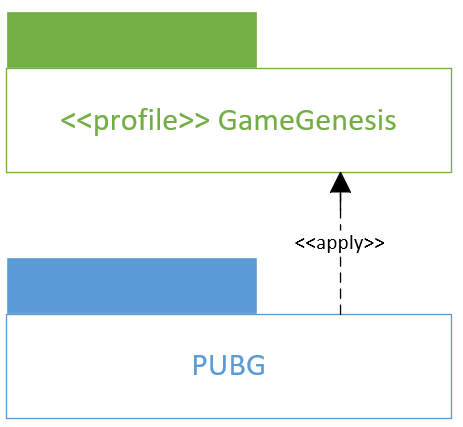
\includegraphics[width=5cm]{10_img/chap6/profile_gg_apply_pubg.PNG}
    \caption{Modélisation de l'application du profil à PUBG}
    \label{fig.racine_stereo}
\end{figure}

\begin{figure}
    \centering
    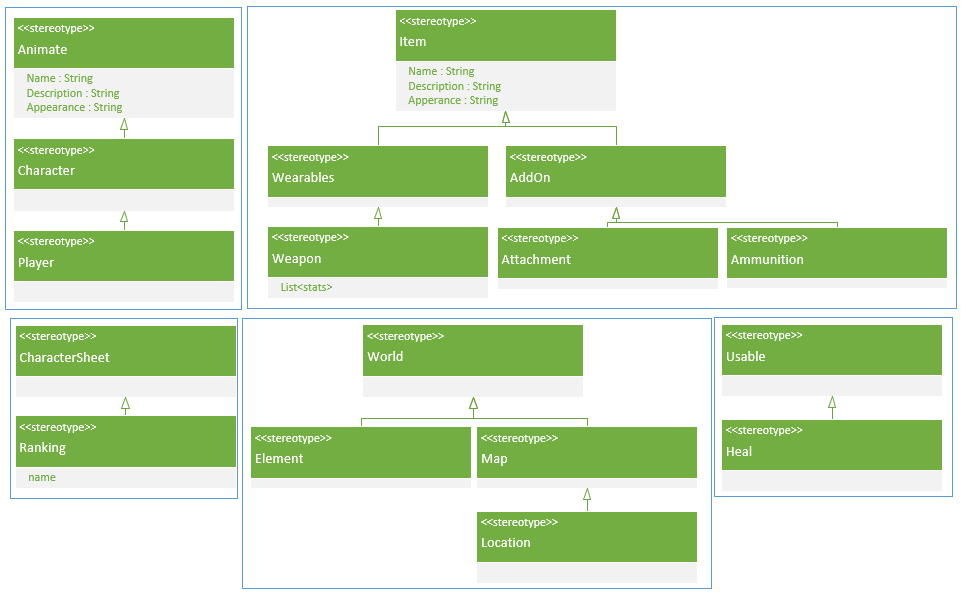
\includegraphics[width=14cm]{10_img/chap6/final_profile.PNG}
    \caption{Les stéréotypes de \emph{Game Genesis} utilisés dans l'exemple}
    \label{fig.racine_stereo}
\end{figure}

%\begin{figure}
%    \centering
%    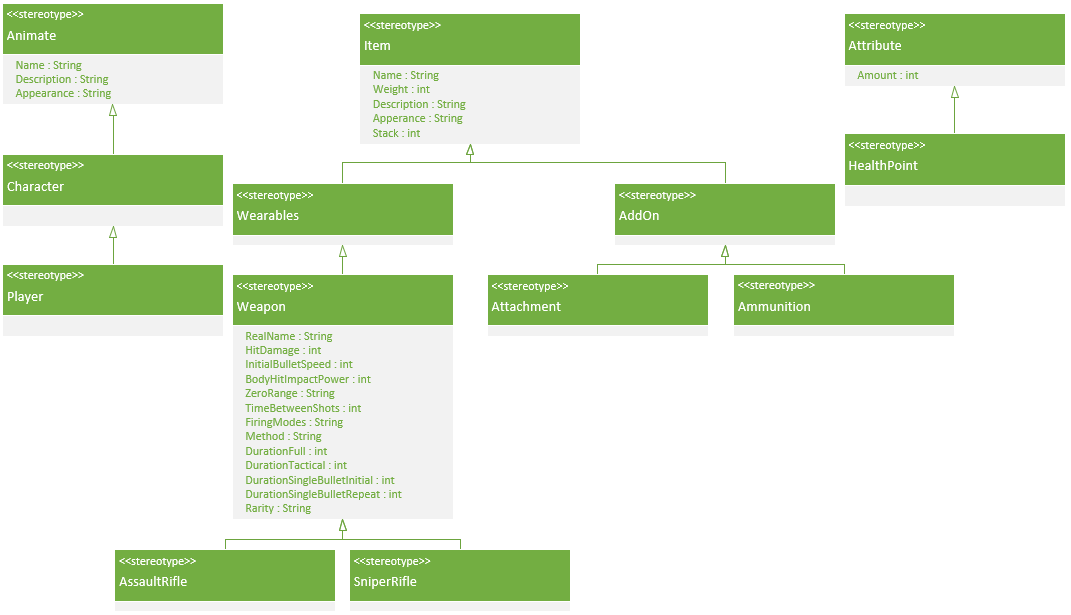
\includegraphics[width=14cm]{10_img/chap6/profile_evo.PNG}
%    \caption{Les stéréotypes modifiés pour l'utilisation pour PUBG.}
%    \label{fig.racine_stereo}
%\end{figure}

Les stéréotypes présents dans \emph{Game Genesis} permettent de classifier les \'el\'ements de \emph{Mechanics} pour la rédaction d'un GDD.
Afin de mieux comprendre le fonctionnement de \emph{Game Genesis}, nous avons extrait une partie du profil et la pr\'esentons dans la Figure~\ref{fig.racine_stereo}.
Cette partie du profil inclut les stéréotypes qui sont utilisés dans les exemples présentés dans la suite du chapitre.
De nombreux attributs ont été ajoutés dans les stéréotypes.
Ceux-ci correspondent aux attributs qui auraient pu être ajoutés par un \emph{game designer} dans le profil.
Ajouter de tels attributs permet d'inclure automatiquement les attributs dans les classes créées à partir du profil UML par l'héritage.


\subsection{La modélisation d'une partie de PUBG}
\begin{figure}[H]
    \centering
    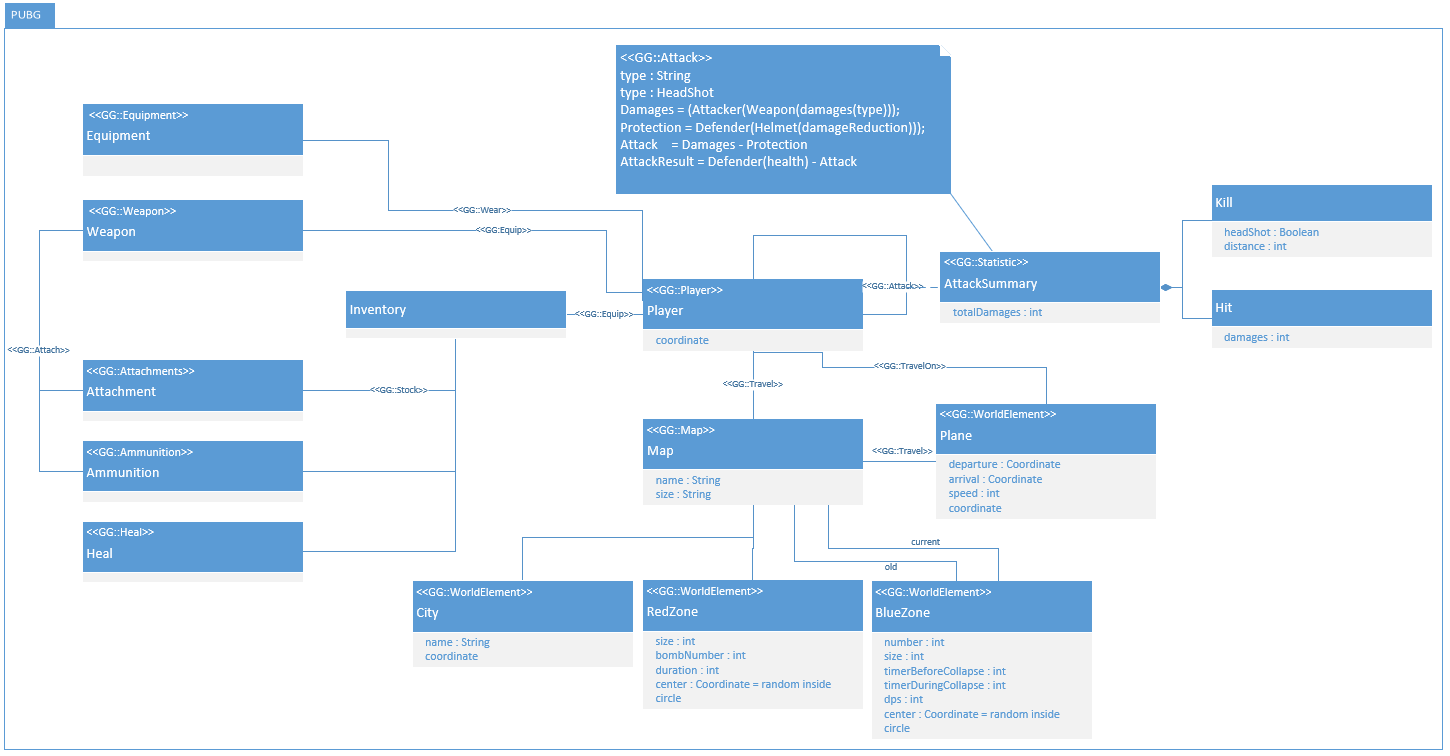
\includegraphics[width=\linewidth]{10_img/chap6/final_model.PNG}
    \caption{Modèle de l'initialisation d'une partie de PUBG.}
    \label{fig.PUBG_model}
\end{figure}

\gt{Figure: je vais revoir cette figure ult\'erieurement! Mais tu
r\'ef\`eres \`a \texttt{Player68} (ou 25) alors que, formellement, n'y
a pas de classe qui porte ce nom.}

La Figure~\ref{fig.PUBG_model} présente l'état d'une partie de PUBG à son initialisation ainsi que les interactions possibles entre les éléments de~\emph{mechanics} présentés.

Cependant décrire l'intégralité du système serait extrêmement long et ne serait pas un apport important pour ce mémoire. Nous allons donc nous concentrer sur certaines parties choisies qui seront décrites plus en détails.

\subsubsection{Représentation des \texttt{item}}

Dans la Figure~\ref{fig.PUBG_model} on voit la présence de cinq classes abstraites : \texttt{Equipment}, \texttt{Weapon}, \texttt{Attachment}, \texttt{Ammunition}, \texttt{Heal}.

Ces éléments sont représentés par des classes abstraites afin de représenter des catégories de classes. Le nombre de classes présentes dans ces catégories est très important et le détail de ces éléments n'est pas essentiel à la compréhension du modèle.

Afin de mieux comprendre le contenu de ces catégories nous allons donner un exemple rapide qui servira à la Section~\ref{sect.attack}.

PUBG est un \emph{Battle Royal} comprenant énormément d'armes différentes. \emph{Game Genesis} classifie ces armes dans la partie \texttt{Weapon}\ref{A-Weapon}. Dans PUBG nous retrouvons des armes catégorisées comme \texttt{SniperRifle}. C'est le cas du \texttt{Kar98k}, du \texttt{M24} et de l'\texttt{AWM}.

Afin de comprendre comment fonctionnent les classes abstraites décrites dans la Figure~\ref{fig.PUBG_model} nous allons représenter le modèle qui amènerait de la classe abstraite (Figure~\ref{fig.abstract_weapon}) vers les trois armes citées précédemment dans la Figure~\ref{fig.example_sniper}.


\begin{figure}
    \centering
    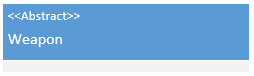
\includegraphics[width=6cm]{10_img/chap6/weap.PNG}
    \caption{La classe abstraite \texttt{Weapon}}
    \label{fig.abstract_weapon}
\end{figure}

\begin{figure}
    \centering
    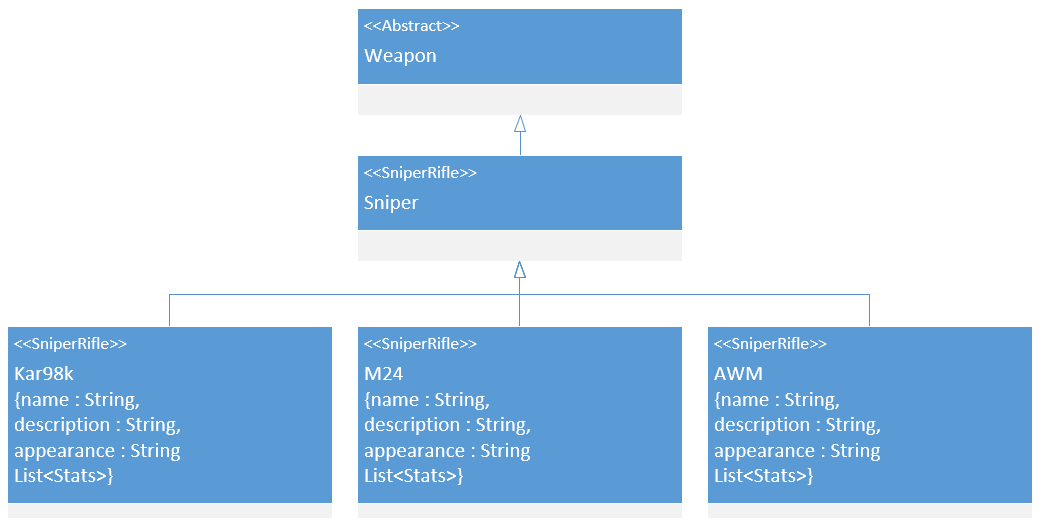
\includegraphics[width=10cm]{10_img/chap6/snipers.PNG}
    \caption{De la classe abstraite \texttt{Weapon} vers les classes de \texttt{SniperRifle} spécifiques}
    \label{fig.example_sniper}
\end{figure}


Pour représenter toutes les armes de PUBG il faudrait reproduire la Figure~\ref{fig.PUBG_kar98} pour l'intégralit des 52 armes présentes dans PUBG.

\begin{figure}[H]
    \centering
    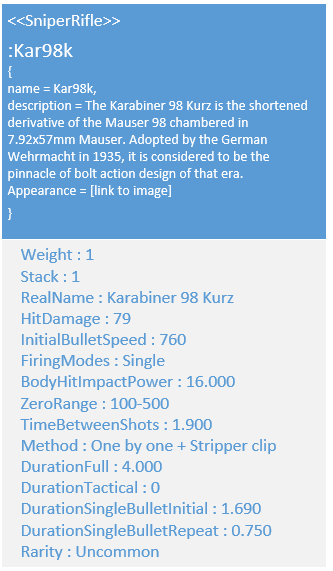
\includegraphics[width=6cm]{10_img/chap6/kar98k.PNG}
    \caption{Représentation finale simulée d'un \texttt{Kar98k} avec ses attributs}
    \label{fig.PUBG_kar98}
\end{figure}




\subsubsection{Un joueur en attaque un autre}
\label{sect.attack}
Dans une partie de PUBG le but ultime pour un joueur est d'éliminer les autres joueurs et de sortir vainqueur en tant que dernier survivant. La notion d'attaque entre joueurs est donc essentielle dans la description des éléments de \emph{mechanics} de PUBG et elle est représentée par une association récursive sur \texttt{Soldier} avec l'interaction \texttt{Attack} (présentée dans la Figure~\ref{fig.PUBG_attack_min}. 

\begin{figure}
    \centering
    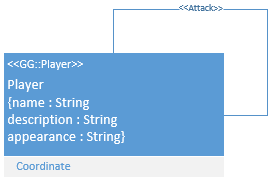
\includegraphics[width=6cm]{10_img/chap6/attack_min.PNG}
    \caption{Un \texttt{Soldier} en attaque un autre.}
    \label{fig.PUBG_attack_min}
\end{figure}

Afin de définir plus précisément l'interaction d'\texttt{Attack} le \emph{game designer} peut décider d'y intégrer des attributs et des méthodes afin de mieux représenter et mieux document la notion d'attaque entre deux joueurs. Par définition une attaque sur PUBG consiste en : un joueur tire sur un autre joueur pour lui faire subir des dégâts.

Afin de calculer ces dégâts, nous avons besoin d'un certain nombre d'informations comme la quantité de dégâts ou les protections possible contre les dégâts.
Dans un FPS, il également est possible d'avoir plusieurs types de dégâts en fonction de l'emplacement de l'attaque.
C'est le cas dans PUBG qui différencie les dégâts en trois types classés du plus fort au moins fort : tête > torse > autres.
Ensuite le calcul des dommages s'effectue en prenant en compte les protections portées par le joueur adverse.
Afin d'exprimer le calcul des dégâts nous avons mis en place la formule suivante :

\begin{figure}[H]
\begin{equation*}
\begin{split}
Damages& = Attacker(Weapon(Damages(Type(Value)))\\
Protection& = Defender(Protection(DamageReduction))\\
Calcul& = Defender(health) - (Damages - Protection)
\end{split}
\end{equation*}
\end{figure}

\gt{Ci-haut pour l'\'equation: si par la suite tu ne r\'ef\`eres pas
explicitement \`a cette \'equation, alors pas besoin de lui donner un
num\'ero et un label.}


\gt{Ci-haut et ci-bas: pas besoin de mettre en guillemets si tu
utilises la police appropri\'ee~: \texttt{Attack}.}

Cette formule de calcul des dégâts est présente dans l'association entre les deux joueurs sur laquelle un stéréotype \texttt{Attack} est appliqué (Figure~\ref{fig.PUBG_attack_min}).

\begin{figure}[H]
    \centering
    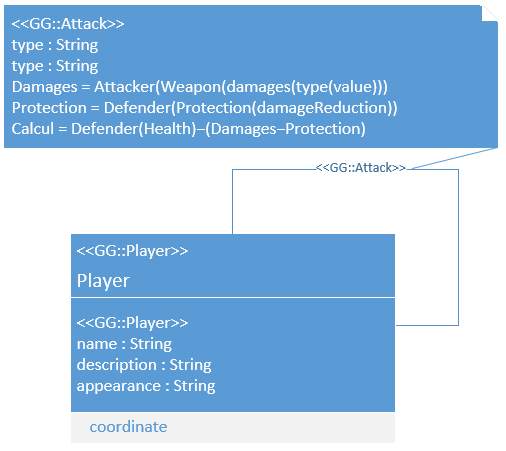
\includegraphics[width=6cm]{10_img/chap6/p_attack_p.PNG}
    \caption{Calcul des dégâts d'une attaque.}
    \label{fig.PUBG_attack_min}
\end{figure}

On considère alors que le \emph{game designer} a modifié le stéréotype \texttt{Attack} de \emph{Game Genesis} afin que toutes les actions d'attaque soient régies par cette formule.

Appliquer ce calcul des dégâts donnerait la simulation suivante :

\begin{table}[H]
\footnotesize
\begin{framed}
Un \texttt{Soldier}, appelé \emph{Soldier25}, possédant une arme de type \texttt{Kar98k} effectue un tir à la tête sur un autre joueur, appelé \emph{Soldier26}, portant un \texttt{HelmetT2}.


\begin{equation*}
\begin{split}
Damages& = Attacker:\texttt{Soldier25}(\texttt{Weapon}:\texttt{Kar98k}(Damages(Type:HeadShot(197.50)))\\
Protection& = Defender:\texttt{Soldier26}(Protection:\texttt{HelmetT2}(DamageReduction:40\%))\\
Calcul& = Defender:\texttt{Soldier26}(Health:100) - (197.50 - (Protection:40\%))\\
Result& = -18.5
\end{split}
\end{equation*}


Dans cet exemple l'attaque génère 118.5 points de dégâts, laissant le \texttt{Soldier26} avec un total de vie de -18.5. Ce total négatif indique la mort du \texttt{Soldier26}.
\end{framed}
\end{table}


La mort du \texttt{Soldier26} si sa vie est inférieure à 0 peut être exprimée par les contraintes suivantes~:

\begin{table}[H]
\footnotesize
\begin{framed}
    Player(health) : is max 100.\\
    (IF Player(health) < 0)\\
    \{\\
    IF Gamemode is "solo" ==> Player is dead and eliminated.\\
    IF Gamemode is "duo" OR "squad" ==> Player is knocked.\\
    \}
\end{framed}
\end{table}






%%%%%%%%%%%%%%%%%%%%%%%%%%%%%%%%%%%%%%%%%%%%%%%%%%%%%%%%%%%%%%%%%%%%%%%%%%%%%%%%%%%%%%%
\begin{comment}

\subsection{La modélisation d'une \AVERIFIER{classe de joueurs avec leurs armes}}


\begin{figure}[H]
    \centering
    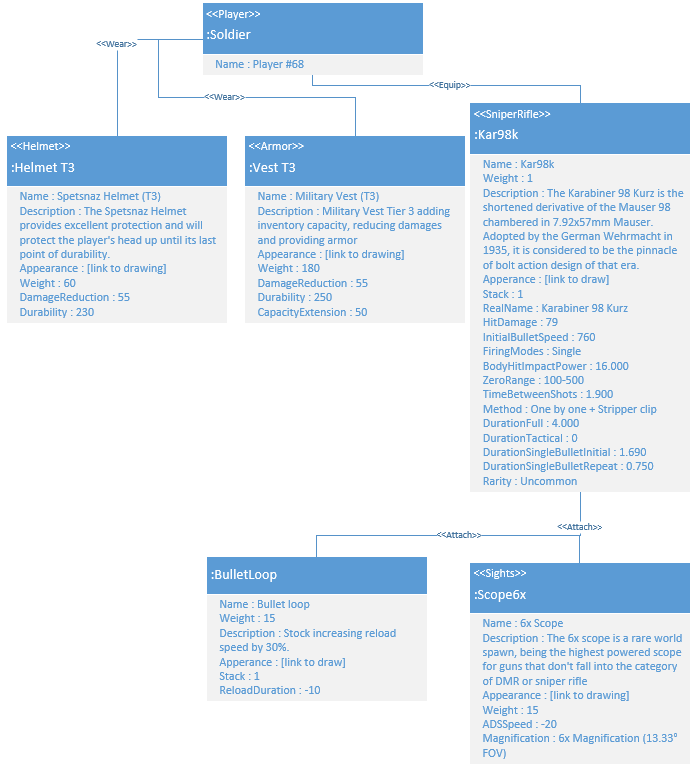
\includegraphics[width=14cm]{10_img/chap6/object_joueur.PNG}
    \caption{La modélisation d'une instance de joueur avec son arme.}
    \label{fig.player+weapon+equip}
\end{figure}


\gt{Dans la figure: tu ne peux pas avoir le nom de classe
\texttt{Player} qui soit en plus st\'er\'eotyp\'e par
<<\texttt{Player}>>.}
\eh{Remplacé par Soldier}

\gt{De plus: Pourquoi Player68?  Comme indiqu\'e ailleurs, avec les
st\'er\'eotypes, tu d\'efinis des classes, et non des instances. Or,
quand on voit <<Name: Player68>>, cela donne vraiment l'impression que
c'est une instance qui est d\'efinie, et non une classe.}

\gt{Et aussi: si tu veux sp\'ecifiers classes st\'er\'eotyp\'es via
des valeurs \'etiquet\'ees, alors ce n'est pas la bonne syntaxe.  Il
faut plut\^ot utiliser la syntaxe 'attribut = valeur' --- le tout (il
me semble) entre accolades.  Revoir les articles UML \`a ce sujet.}

\gt{Ci-bas: il faut rendre plus clair, plus explicite, le fait que
c'est une classe de joueurs qui est mod\'elis\'ee, et non un joeur
sp\'ecifique. Parce qu'un st\'er\'eotype sert \`a d\'efinir/d\'ecrire
des {\bf classes} et non des {\bf instances}. Les st\'er\'eotypes sont
utilis\'es dans un mod\`ele de jeu, et non dans une instance
sp\'ecifique du jeu en cours d'ex\'ecution.}

La Figure~\ref{fig.player+weapon+equip} présente la modélisation d'un joueur.
Celui-ci est équipé d'un casque \texttt{Tier3} et d'une veste \texttt{T3}.
Il est armé d'un fusil \emph{sniper} de type \texttt{Kar98k} lui même équipe d'une lunette \texttt{Scope6x} et d'une ceinture de munitions.

\gt{Si possible, il serait pr\'ef\'erable que Equip soit attach\'e \`a
un endroit diff\'erent de Wear.  C'est ok il me semble de mettre
plusieurs fois des instances de la m\^eme association sur une m\^eme
ligne, mais moins de mettre une association compl\`etement
diff\'erente!}

\gt{De plus, il me semble que dans les exemples vus \`a diff\'erents
endroits, le nom d'une association st\'er\'eotyp\'ee doit aussi \^etre
entre chevrons, <<Wear>>, <<Equip>>, etc.}

Comme décrit \`a la Section~\ref{sect.gg_what}, nous avons utilisé des classes afin de représenter les éléments du jeu, alors que des associations entre classes représentent les interactions possibles entre éléments du jeu.
Sur ces classes et associations, nous avons appliqué les stéréotypes du profil \emph{Game Genesis} afin de pouvoir classifier et spécialiser les différents éléments modélisés.

\end{comment}
%%%%%%%%%%%%%%%%%%%%%%%%%%%%%%%%%%%%%%%%%%%%%%%%%%%%%%%%%%%%%%%%%%%%%%%%%%%%%%%%%%%%%%%









\section{Conclusion}
